\section{Teoreetiline taust}\label{taust}

Abstraktne masin annab formaliseeritud kirjelduse sellest, millises olekus programm parasjagu asub ja kuidas ühe instruktsiooni täitmine seda olekut muudab~\cite{wilhelm_imperative_2010}. Selline kirjeldus sobib kompilaatori väljundi süstemaatiliseks analüüsiks~\cite{mogensen_introduction_2024}. Käesolevas töös on oluline, et funktsioonikutsete lisamine mõjutab kogu täitmiskeskkonna käitumist, sealhulgas täitmisraamide haldust, argumentide edastamist ja kontrollivoo taastamist~\cite{mogensen_programming_2026}. Esmalt antakse ülevaade abstraktsete masinate rollist. Seejärel kirjeldatakse \textsc{CMa} arhitektuuri, võrreldakse levinud virtuaalsete täitmismudelitega. Lõpuks seotakse lähtekohad funktsioonikutsete mõiste ja kasutusloogikaga.

\subsection{Abstraktsed masinad kompilaatorites}\label{taust:abstraktsed}

Abstraktne masin on formalism, milles programmi täitmist kirjeldatakse piiratud hulga olekute ja üleminekureeglite abil~\cite{wilhelm_imperative_2010}. Tüüpiliselt koosneb selline mudel käsustikust, mälust ning semantilisest kirjeldusest, mis määrab, kuidas ühe käsu täitmine muudab masina olekut. Lähenemine võimaldab eraldada programmitäitmise loogika konkreetse riistvara detailidest, säilitades samas mõisted, mis on kompilaatorite mõistmisel keskse tähtsusega~\cite{mogensen_introduction_2024}.

Kompilaatorite kontekstis kasutatakse abstraktseid masinaid sageli vahekihina lähtekeele ja sihtplatvormi vahel~\cite{wilhelm_compiler_2013}. Õppetöös seisneb abstraktsete masinate tugevus selles, et need teevad nähtavaks protsessid, mis reaalses süsteemis jäävad sageli peidetuks optimeerimiste või riistvaraliste abstraktsioonide taha. \textsc{CMa} pakub käesoleva töö jaoks sobiva tasakaalu, kuna see on piisavalt lihtne ja väljendusrikas, et modelleerida funktsioonikutseid ja lokaalset mälu~\cite{wilhelm_imperative_2010}.

\subsection{\textsc{CMa} arhitektuur}\label{taust:CMa}

Käesolevas töös käsitletav \textsc{CMa} on pinu- ja käsupõhine abstraktne masin, mille eesmärk on teha imperatiivse programmi täitmise mehhanism paremini jälgitavaks. Masin on esitatud Wilhelm ja Seidli teoses~\cite{wilhelm_imperative_2010}. Masina seisundit saab kirjeldada väikese hulga selgete komponentide kaudu: programmiloendur määrab järgmise täidetava käsu, pinu hoiab vaheväärtusi ja täitmisraamidega seotud andmeid ning kuhjamälu (ingl \emph{heap}\footnote{\url{https://akit.cyber.ee/term/9959-heap}}) võimaldab modelleerida dünaamiliselt hallatavat mälu~\cite{wilhelm_imperative_2010}.

\textsc{CMa} arhitektuuri mõistmine on käesoleva töö seisukohalt keskne, kuna funktsioonikutsete toe lisamine puudutab korraga nii käsustiku semantikat kui ka väljakutsete elutsüklit. Kui juhtimine antakse ühelt protseduurilt teisele, tuleb salvestada tagasipöördumisaadress, siduda argumendid õige täitmisraamiga ning taastada pärast alamprogrammi lõppu eelnev täitmiskontekst~\cite{mogensen_programming_2026}. Järgmistes alajaotustes kirjeldatakse seetõttu eraldi \textsc{CMa} mälumudelit ning käsustikku, sest nende kokkupuutepunktis hakkab funktsioonikutsete laiendus masina käitumist muutma.

\subsubsection{Mälu, registrid ja funktsiooniraamistik}\label{taust:CMa:malu}

\textsc{CMa} mälumudeli keskmes on pinu, kuhi ja väike hulk juhtimisega seotud registreid, mille koosmõju määrab, kuidas programm parasjagu edeneb ja millises kontekstis käske täidetakse~\cite{wilhelm_imperative_2010}. Pinu toimib tööalana vaheväärtuste, argumentide, lokaalse oleku ja tagasipöördumisega seotud andmete hoidmiseks~\cite{mogensen_programming_2026}. Kuhi eristub pinust selle poolest, et modelleerib pikema elueaga andmeid, mille kasutus ei ole otseselt seotud ühe konkreetse täitmisraami kestusega~\cite{gabbrielli_programming_2023}. Selline tööjaotus aitab selgelt eristada ajutist arvutusolekut ja püsivamat mälukasutust.

Juhtimise seisukohalt on keskne programmiloendur, mis osutab parasjasti täidetavale või järgmisena täitmisele minevale käsule~\cite{wilhelm_imperative_2010}. Kui aritmeetiline või andmete teisendamisega seotud käsk muudab peamiselt pinu sisu, siis juhtvoogu muutvad käsud mõjutavad lisaks programmiloendurit ning sellega kogu täitmistee struktuuri~\cite{seidl_compiler_2012}. Funktsioonikutsete seisukohalt on oluline raamipõhine adresseerimine: väljakutse alustamisel seotakse uus täitmiskontekst kindla raami külge ning selle raami suhtes tõlgendatakse lokaalseid muutujaid ja parameetreid~\cite{mogensen_programming_2026}. Nii välditakse olukorda, kus eri alamprogrammide lokaalne olek seguneb.

Järgnevalt on esitatud Wilhelm ja Seidli~\cite{wilhelm_imperative_2010} käsitluses esinevad tähised ning seletused olulistele registritele:

\begin{itemize}
	\item C (ingl \emph{program store}) tähistab käskude ala ehk seda mälupiirkonda, kus paikneb täidetav \textsc{CMa} programm. Piirkonnas asuvad masina instruktsioonid järjestatult aadresside järgi.
	\item S (ingl \emph{program memory}) on tööala, milles alumistel aadressidel paiknevale pinule paigutatakse vaheväärtused, argumendid, lokaalsed muutujad ja funktsioonikutsetega seotud andmed. Piirkond muutub avaldiste hindamisel ja täitmisraamide loomisel enim.
	\item PC (ingl \emph{program counter}) ehk programmiloendur osutab käsualas C sellele instruktsioonile, mida parasjagu täidetakse või mis täidetakse järgmisena. Juhtvoogu muutvad käsud muudavad PC väärtust ning seeläbi kogu programmi täitmisteed.
	\item IR (ingl \emph{instruction register}) ehk käsuregister hoiab käsualast loetud instruktsiooni, mida masin parajasti tõlgendab ja täidab. Register seob käsu lugemise ja järgneva täitmise üheks tervikuks.
	\item SP (ingl \emph{stack pointer}) ehk pinuviit osutab pinu S aktiivsele tipule või järgmisele vabale kohale, sõltuvalt konkreetsest operatsioonist. Registri abil on võimalik määrata, kuhu uus väärtus pinus paigutatakse ja milliselt kohalt olemasolev väärtus loetakse.
	\item FP (ingl \emph{frame pointer}) osutab aktiivse täitmisraami ankrukohale, mille suhtes aadresseeritakse parameetreid ja lokaalseid muutujaid. Funktsioonikutse ajal võimaldab see eristada eri väljakutsete andmeid ka siis, kui pinu kõrgus muutub.
	\item HP (ingl \emph{heap pointer}) tähistab kuhja piiri, viidates kõige alumisele elemendile, ja aitab jälgida, et pinu kasv ei satuks dünaamiliselt hallatava mäluga konflikti.
	\item EP (ingl \emph{extreme pointer}) märgib piiri, milleni aktiivne väljakutse võib pinu kasvatada ilma kuhjaga kokku põrkamata. Seda kasutatakse funktsioonikutse järel, kui tuleb kontrollida, kas uue täitmisraami jaoks on piisavalt ruumi.
\end{itemize}

Joonisel~\ref{fig:CMa-malujaotus} on kujutatud \textsc{CMa} põhiline mälujaotus: programmimälu C, kust masin loeb täidetavaid käske, ning töömälu S, milles paiknevad nii pinu kui ka kuhi.

\begin{figure}[H]
	\centering
	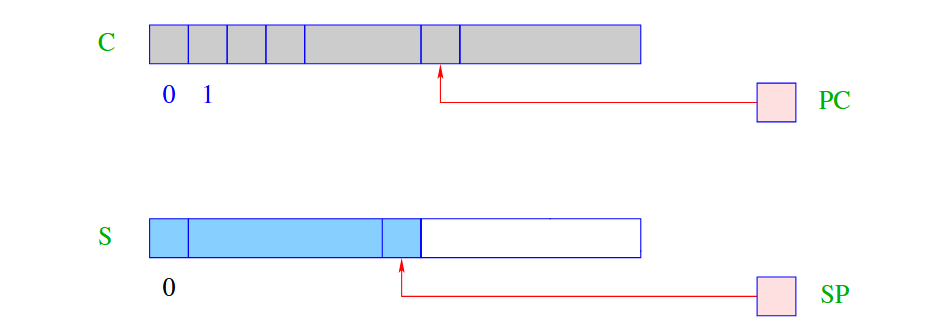
\includegraphics[width=0.82\textwidth]{estonian/joonised/malujaotus.png}
	\caption{\textsc{CMa} mälujaotus ja seotud registrid~\cite{wilhelm_imperative_2010}}\label{fig:CMa-malujaotus}
\end{figure}

Täitmisraam koondab tüüpiliselt vähemalt parameetrite, lokaalsete muutujate ja tagasipöördumiseks vajaliku metaandmestiku~\cite{gabbrielli_programming_2023}. Kui programm kutsub välja järgmise funktsiooni, luuakse uus raam olemasoleva raami peale ning lõpetamisel taastatakse eelmine kontekst~\cite{mogensen_programming_2026}. Mehhanism muudab võimalikuks pesastatud väljakutsed, rekursiooni ja kontrollitud tagasipöördumise. \textsc{CMa} puhul on eelnev oluline, sest käesoleva töö laiendus peab säilitama raamide korrektsuse ka siis, kui väljakutsed lisanduvad algselt lihtsamale täitmismudelile.

\subsubsection{Põhilisemad käsud ja nende täitmissemantika}\label{taust:CMa:kasustik}

\textsc{CMa} käsustiku võib vaadelda kui reeglistikku, mille iga käsk teisendab masina seisundit etteantud viisil~\cite{wilhelm_imperative_2010}. Semantilises mõttes ei ole käsk üksnes süntaktiline märge, vaid operatsioon, mille täitmisel muutuvad pinu sisu, registrid või juhtvoog. Alljärgnevalt on olemasolevad põhikäsud esitatud kompaktse koondtabelina (tabel~\ref{tab:CMa-pohikasud}), mis annab ülevaate andme-, aritmeetika-, loogika- ja juhtvookäskude semantikast. Funktsioonikutsete käskude detailne kirjeldus järgneb eraldi alajaotuses.

\begin{table}[H]
\centering
\footnotesize
\caption{Olemasolevad \textsc{CMa} põhikäsud ja nende semantika~\cite{wilhelm_imperative_2010}}\label{tab:CMa-pohikasud}
\begin{tblr}{
  colspec = {l l l},
  row{1} = {font=\bfseries},
  hline{1,2,Z} = {0.8pt},
}
Käsk          & Semantika                                                        & Rühm \\
\texttt{loadc q}  & \texttt{SP <- SP+1; S[SP] <- q}                          & andmed \\
\texttt{load}     & \texttt{S[SP] <- S[S[SP]]}                               & andmed \\
\texttt{store}    & \texttt{S[S[SP]] <- S[SP-1]; SP <- SP-1}                 & andmed \\
\texttt{loada q}  & \texttt{= loadc q; load}                                 & andmed \\
\texttt{storea q} & \texttt{= loadc q; store}                                & andmed \\
\texttt{mul}      & \texttt{S[SP-1] <- S[SP-1] * S[SP]; SP <- SP-1}         & aritmeetika \\
\texttt{neg}      & \texttt{S[SP] <- -S[SP]}                                 & aritmeetika \\
\texttt{leq}      & \texttt{S[SP-1] <- (S[SP-1] <= S[SP]); SP <- SP-1}      & loogika \\
\texttt{dup}      & \texttt{S[SP+1] <- S[SP]; SP <- SP+1}                   & pinu \\
\texttt{pop}      & \texttt{SP <- SP-1}                                      & pinu \\
\texttt{jump A}   & \texttt{PC <- A}                                         & juhtvoog \\
\texttt{jumpz A}  & \texttt{kui S[SP]=0: PC <- A; SP <- SP-1}                & juhtvoog \\
\texttt{jumpi A}  & \texttt{PC <- A + S[SP]; SP <- SP-1}                     & juhtvoog \\
\end{tblr}
\end{table}

Andmekäsud laadivad väärtusi pinule (\verb|loadc|, \verb|load|, \verb|loada|) või salvestavad neid mällu (\verb|store|, \verb|storea|). Binaarsed aritmeetika- ja loogikakäsud (\verb|mul|, \verb|leq| jt) tarbivad pinust kaks pealmist väärtust ja asetavad tulemuse asemele. Unaarsed (\verb|neg|, \verb|not|) muudavad ainult tippu. Sama muster kehtib käskudele \verb|add|, \verb|sub|, \verb|div|, \verb|mod|, \verb|and|, \verb|or|, \verb|eq|, \verb|neq|, \verb|le|, \verb|gr| ja \verb|geq|~\cite{wilhelm_imperative_2010}. Juhtvookäsud \verb|jump|, \verb|jumpz| ja \verb|jumpi| muudavad programmiloendurit. Viimane on vajalik lülituskonstruktsioonide jaoks, kus sihtaadress sõltub pinu tipus olevast väärtusest.

\subsubsection{Funktsioonikutsete käsud ja nende täitmissemantika}\label{taust:CMa:valjakutse}

Funktsioonikutsete seisukohalt on kõige olulisemad käsud, mis valmistavad ette uue väljakutse, loovad täitmisraami ja tagavad kontrollitud tagasipöördumise~\cite{mogensen_programming_2026}. Kui sildid märgivad lihtsalt käsuala sihtkohti, siis funktsioonid koondavad selliste sihtkohtade ümber korduvkasutatava käsujada, millele saab üle anda juhtimise koos argumentide ja hilisema tagasipöördumise kokkuleppega~\cite{wilhelm_imperative_2010}. Nende käskude mõistmiseks on oluline pidada meeles jaotises~\ref{taust:CMa:malu} kirjeldatud registreid FP, HP ja EP. Lisaks kasutatakse allolevas pseudokoodis abimuutujat \verb|tmp| tagasipöördumisaadressi ajutiseks hoidmiseks ja loendurit \verb|i| käsu \verb|slide| sisemise kopeerimistsükli kirjeldamiseks. Need ei ole eraldi masina registrid, vaid pseudokoodi abivahendid.

Esimese rühma moodustavad käsud, mis loovad täitmisraami ja annavad juhtimise üle kutsutavale funktsioonile. Käskude semantika on esitatud järgmises pseudokoodiplokis:

\begin{minted}{text}
mark     :  S[SP + 1] <- EP
            S[SP + 2] <- FP
            SP <- SP + 2

call     :  FP <- SP
            tmp <- PC
            PC <- S[SP]
            S[SP] <- tmp

enter m  :  EP <- SP + m
            if EP >= HP then error("Stack Overflow")

alloc m  :  SP <- SP + m
\end{minted}

Käsk \verb|mark| valmistab raamatu~\cite{wilhelm_imperative_2010} järgi ette uue täitmisraami, salvestades pinule eelmise EP ja FP väärtuse. Sisuliselt loob see pinule uue väljakutse jaoks administratiivse raami alguse, kuhu on talletatud seni aktiivse raami olulised piirid — hiljem võimaldab see kutsutud funktsioonist korrektselt tagasi pöörduda ja taastada eelmine täitmiskontekst. Olekumuutust visualiseerib joonis~\ref{fig:CMa-mark}:

\begin{figure}[H]
	\centering
	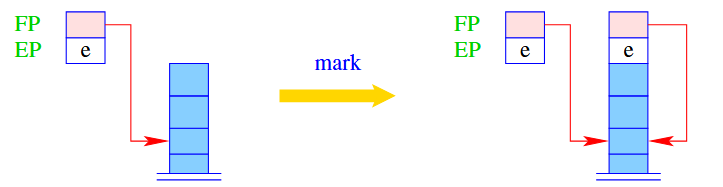
\includegraphics[width=0.75\textwidth]{estonian/joonised/mark.png}
	\caption{Käsu \texttt{mark} mõju pinule~\cite{wilhelm_imperative_2010}}\label{fig:CMa-mark}
\end{figure}

Käsk \verb|call| annab juhtimise üle kutsutavale funktsioonile. Praegusest pinuviida asukohast saab uue aktiivse raami ankur, senine PC salvestatakse tagasipöördumisaadressina ning täitmine jätkub kutsutava funktsiooni algusest. Nii muudetakse pinu tipus olnud sihtaadress tagasipöördumiseks vajalikuks infoks, ilma et oleks vaja luua eraldi kõrvalstruktuuri. Juhtimise üleandmist visualiseerib joonis~\ref{fig:CMa-call}:

\begin{figure}[H]
	\centering
	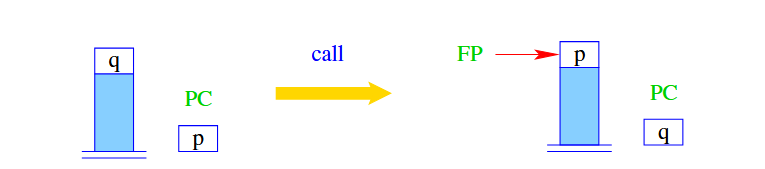
\includegraphics[width=0.75\textwidth]{estonian/joonised/call.png}
	\caption{Käsu \texttt{call} mõju raamile, programmiloendurile ja pinule~\cite{wilhelm_imperative_2010}}\label{fig:CMa-call}
\end{figure}

Käsk \verb|enter m| määrab, kui suureks võib aktiivse funktsiooni tööala pinus kasvada: EP nihutatakse ettepoole ja kontrollitakse kohe, kas selline kasv oleks kuhjapiiriga kooskõlas. Siin tähistab \verb|m| nende pinukohtade arvu, mida funktsioon vajab oma lokaalsete andmete ja vahetulemuste jaoks — käsk ei paiguta neid väärtusi veel pinule, vaid reserveerib ruumi ja tagab, et see ruum ei kattu kuhjaga. Ruumikontrolli visualiseerib joonis~\ref{fig:CMa-enter}:

\begin{figure}[H]
	\centering
	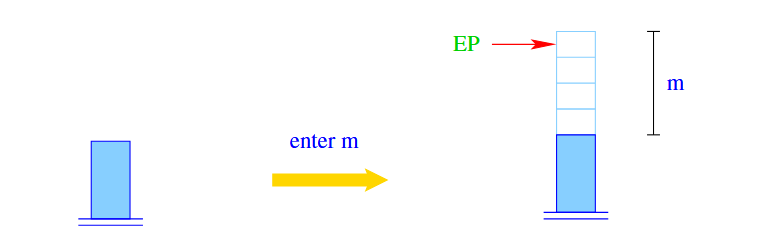
\includegraphics[width=0.75\textwidth]{estonian/joonised/enter.png}
	\caption{Käsu \texttt{enter m} mõju registrile EP ja mälupiirile~\cite{wilhelm_imperative_2010}}\label{fig:CMa-enter}
\end{figure}

Käsk \verb|alloc m| nihutab pinuviida reaalselt edasi ja teeb reserveeritud kohad kasutatavaks. Seega moodustavad \verb|enter m| ja \verb|alloc m| koos loogilise paari: esimene kontrollib piire, teine realiseerib ruumi broneerimise pinus. Muutust visualiseerib joonis~\ref{fig:CMa-alloc}:

\begin{figure}[H]
	\centering
	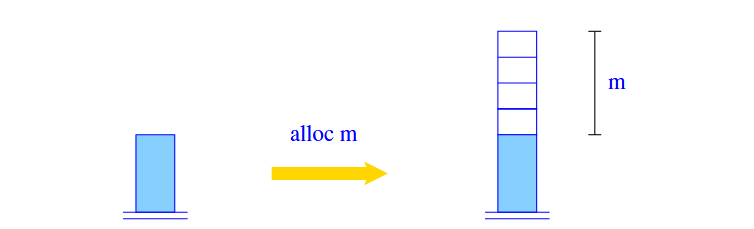
\includegraphics[width=0.75\textwidth]{estonian/joonised/alloc.png}
	\caption{Käsu \texttt{alloc m} mõju pinuviidale~\cite{wilhelm_imperative_2010}}\label{fig:CMa-alloc}
\end{figure}

Teise rühma moodustavad käsud, mis tegelevad raamipõhise adresseerimise ja mitmeväärtuslike mäluoperatsioonidega. Nende abil saab funktsiooni sees pöörduda parameetrite ja lokaalsete muutujate poole raami suhtes ning lugeda või kirjutada korraga mitut järjestikust pinukohta. Nende käskude semantika on esitatud järgmises pseudokoodiplokis:

\begin{minted}{text}
loadrc j :  SP <- SP + 1
            S[SP] <- FP + j

load m   :  target <- S[SP]
            for i = m - 1 downto 0 do
                S[SP + i] <- S[target + i]
            SP <- SP + m - 1

store m  :  target <- S[SP]
            for i = 0 to m - 1 do
                S[target + i] <- S[SP - m + i]
            SP <- SP - 1

loadr j m  = loadrc j; load m
storer j m = loadrc j; store m
\end{minted}

Käsk \verb|loadrc j| asetab pinu tippu aktiivse raami ankuraadressi, millele on liidetud nihe \verb|j|. Seega annab see raamipõhise adresseerimise: \verb|FP + j| osutab konkreetsele kohale aktiivses täitmisraamis, kus paiknevad parameetrid või lokaalsed muutujad. Käsud \verb|loadr j m| ja \verb|storer j m| on tuletatud käsud, mis ühendavad \verb|loadrc| abil saadud FP arvutamise ja järgnevate mäluoperatsioonide üheks lühemaks vormiks: \verb|loadr j m| on samaväärne käsupaari \verb|loadrc j| ja \verb|load m| järjestikuse täitmisega ning \verb|storer j m| on samaväärne käsupaari \verb|loadrc j| ja \verb|store m| järjestikuse täitmisega~\cite{wilhelm_imperative_2010}.

Käsk \verb|load m| loeb pinu tipus olevalt aadressilt \verb|m| järjestikust väärtust ja asetab need pinule — pinu kasvab seega \verb|m - 1| elemendi võrra, kuna aadress asendatakse loetud väärtustega. Olekumuutust visualiseerib joonis~\ref{fig:CMa-loadm}:

\begin{figure}[H]
	\centering
	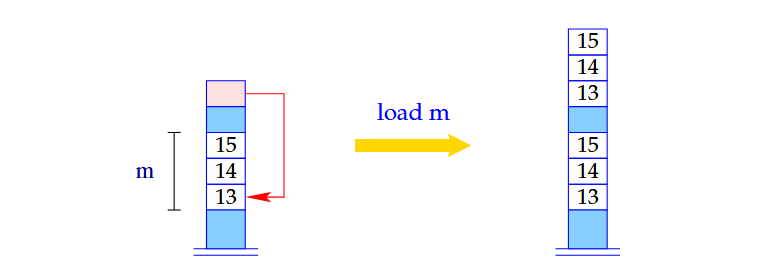
\includegraphics[width=0.75\textwidth]{estonian/joonised/loadm.png}
	\caption{Käsu \texttt{load m} mõju pinule~\cite{wilhelm_imperative_2010}}\label{fig:CMa-loadm}
\end{figure}

Käsk \verb|store m| kirjutab \verb|m| pinu tipus olevat väärtust pinu tipus olevale sihtaadressile ning eemaldab seejärel sihtaadressi pinust. Nii säilivad pinul kirjutatud väärtused, kuid aadress eemaldatakse. Olekumuutust visualiseerib joonis~\ref{fig:CMa-storem}:

\begin{figure}[H]
	\centering
	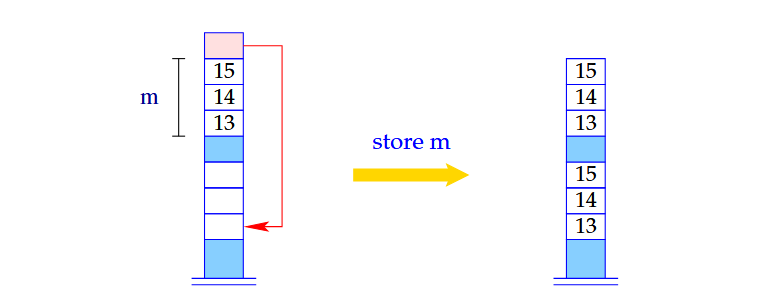
\includegraphics[width=0.75\textwidth]{estonian/joonised/storem.png}
	\caption{Käsu \texttt{store m} mõju pinule~\cite{wilhelm_imperative_2010}}\label{fig:CMa-storem}
\end{figure}

Kolmanda rühma moodustavad pinu korrastamise ja tagasipöördumisega seotud käsud, mis vastutavad funktsiooni lõpetamise ja väljakutsuja konteksti taastamise eest. Nende käskude semantika on esitatud järgmises pseudokoodiplokis:

\begin{minted}{text}
slide q m :  if q > 0 then
                 if m = 0 then SP <- SP - q
                 else
                     SP <- SP - q - m
                     for i = 0 to m - 1 do
                         SP <- SP + 1
                         S[SP] <- S[SP + q]

return q  :  PC <- S[FP]
             EP <- S[FP - 2]
             if EP >= HP then error("Stack Overflow")
             SP <- FP - q
             FP <- S[FP - 1]
\end{minted}

Käsk \verb|slide q m| korrastab pinu pärast funktsiooni täitmist nii, et \verb|m| tulemusväärtust säilib, kuid \verb|q| eemaldatavat elementi nende alt kaotatakse. Kui säilitatavaid väärtusi ei ole, piisab pinuviida lihtsast tagasinihutamisest. Vastasel juhul tuleb soovitud väärtused nihutada üle eemaldatavate argumentide uude õigesse asukohta. Korrastusmehhanismi visualiseerib joonis~\ref{fig:CMa-slide}:

\begin{figure}[H]
	\centering
	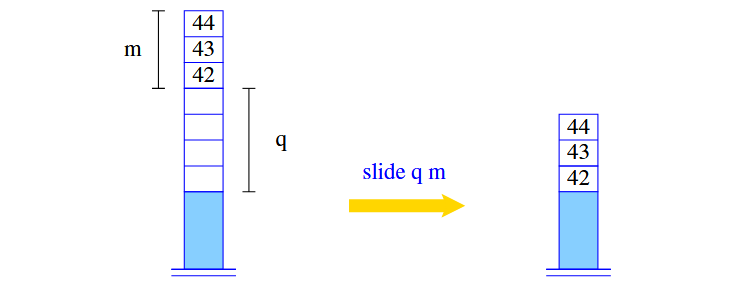
\includegraphics[width=0.8\textwidth]{estonian/joonised/slide.png}
	\caption{Käsu \texttt{slide q m} mõju pinu korrastamisel~\cite{wilhelm_imperative_2010}}\label{fig:CMa-slide}
\end{figure}

Käsk \verb|return q| lõpetab aktiivse funktsiooni täitmise ja taastab väljakutsuja juhtimiskonteksti. Siin tähistab \verb|q| nende tulemuselementide arvu, mis peavad tagasipöördumisel pinule alles jääma. Kõigepealt võetakse aktiivsest raamist tagasipöördumisaadress ja taastatakse eelnevalt salvestatud EP, seejärel kontrollitakse kuhjapiiriga kooskõla, nihutatakse SP tagasi nii et vajalik arv tulemusväärtusi säilib, ja lõpuks taastatakse eelmise väljakutse FP. Sedaviisi koondab \verb|return q| ühte käsku nii juhtimise tagastamise kui ka täitmisraami kokkupakkimise. Tagasipöördumist visualiseerib joonis~\ref{fig:CMa-return}:

\begin{figure}[H]
	\centering
	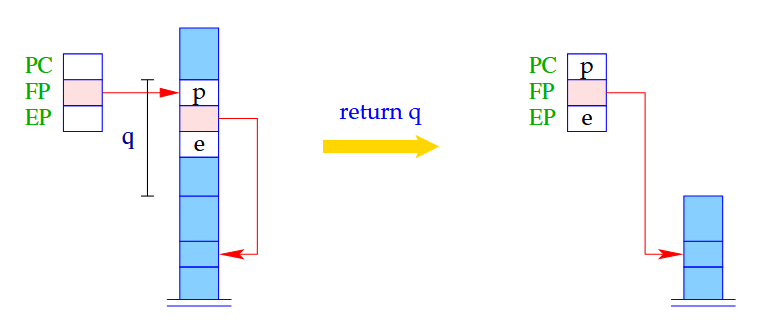
\includegraphics[width=0.8\textwidth]{estonian/joonised/return.png}
	\caption{Käsu \texttt{return q} mõju tagasipöördumisel~\cite{wilhelm_imperative_2010}}\label{fig:CMa-return}
\end{figure}

Koos vaadelduna moodustavad need käsud tervikliku väljakutsetsükli: esmalt salvestatakse eelmine kontekst (\verb|mark|), seejärel antakse juhtimine üle kutsutavale funktsioonile (\verb|call|), kontrollitakse ja reserveeritakse vajalik tööruum (\verb|enter|, \verb|alloc|), adresseeritakse parameetreid ja lokaalseid muutujaid raamipõhiselt (\verb|loadrc|, \verb|load m|, \verb|store m|, \verb|loadr|, \verb|storer|) ning lõpuks korrastatakse pinu ja taastatakse juhtimine (\verb|slide|, \verb|return|). See mehhanism teeb võimalikuks pesastatud väljakutsed ja raamipõhise adresseerimise, millele käesoleva töö praktiline laiendus hiljem toetub.

\subsubsection{Täitmistsükkel}\label{taust:CMa:taitmistsukkel}

\textsc{CMa} täitmistsüklit saab kirjeldada korduva mustrina, milles masin loeb programmiloenduri järgi järgmise käsu, tõlgendab selle tähenduse ning rakendab vastava olekumuutuse~\cite{wilhelm_imperative_2010}. Pärast käsu täitmist uuendatakse programmiloendurit kas järgmise järjestikuse käsu suunas või hüppeliselt, kui käsu semantika seda nõuab~\cite{seidl_compiler_2012}. Selline loe-tõlgenda-täida tsükkel on abstraktse masina tasandil oluline, sest selle abil seotakse üksikud instruktsioonid terviklikuks programmikäitumiseks.

Põhimõtet saab esitada ka lihtsustatud pseudokoodina, kus igal iteratsioonil loetakse käsualast järgmine instruktsioon, salvestatakse see käsuregistrisse IR (ingl \emph{instruction register}), suurendatakse programmiloendurit ning täidetakse loetud käsk~\cite{wilhelm_imperative_2010}. Järgmine näide esitab kirjeldatud tsükli kompaktse kuju.

\begin{minted}{javascript}
while (true) {
  IR <- C[PC];
  PC++;
  execute(IR);
}
\end{minted}

Funktsioonikutsete kontekstis muutub täitmistsükkel oluliseks, kui üks käsk ei piirdu ainult kohaliku andmemuudatusega, vaid avab uue täitmiskonteksti~\cite{mogensen_programming_2026}. Sellisel juhul peab masin säilitama piisavalt infot, et pärast kutsutava koodi lõpetamist saaks täitmist jätkata õigest kohast.

Teoses~\cite{wilhelm_imperative_2010} kirjeldatakse ka koodi genereerimise printsiipe, sealhulgas avaldiste väärtuste ja aadresside (\emph{R-value/L-value}) arvutamist ning aadresskeskkonna kasutamist muutujate sidumiseks mäluaadressidega. Need mõisted on olulised kompilaatori ehitamisel, kuid käesoleva töö skoop piirdub interpretaatori laiendamisega, mistõttu siinkohal pikem käsitlus ei ole vajalik.

\subsection{Sarnased abstraktsed masinad}\label{taust:sarnased}

\textsc{CMa} eripära paremini mõistmiseks on kasulik võrrelda seda kahe levinud täitmismudeliga. Java virtuaalmasin (lühendatult \textsc{Jvm}\footnote{\url{https://docs.oracle.com/javase/specs/jvms/se25/html/index.html}}) kasutab sarnaselt \textsc{CMa}-le pinupõhist täitmismudelit ja meetodiraame, kuid sisaldab lisaks dünaamilist klasside laadimist, verifitseerimist ja erandikäsitlust ning on mõeldud tööstusliku käituskeskkonnana. \textsc{Llvm} IR\footnote{\url{https://llvm.org/docs/LangRef.html}} on omakorda madala taseme vaheesitus, mis toetab analüüsi, optimeerimisi ja mitmele arhitektuurile suunatud koodi genereerimist. Nende kahe tuntuma lahenduse kõrval paistab \textsc{CMa} silma oma lihtsustatud kujuga, mis võimaldab keskenduda täitmisloogikale ilma suure käituskeskkonna lisakeerukuseta.

\subsection{Funktsioonikutsed programmeerimises}\label{taust:funktsioonikutsed}

Funktsioonikutse on mehhanism, mille abil antakse programmi juhtimine ühelt alamprogrammilt teisele, edastatakse argumendid ja valmistatakse ette uus täitmiskontekst~\cite{gabbrielli_programming_2023}. Funktsioonikutse lõppedes tuleb taastada eelnev juhtseis, sealhulgas tagasipöördumisaadress ja väljakutsuja lokaalne keskkond~\cite{mogensen_programming_2026}. See teeb funktsioonikutsetest ühe keskse teema nii programmeerimiskeelte semantikas kui ka virtuaalmasinate ehituses. 

Funktsioonikutsete realiseerimisel kasutatakse Wilhelm ja Seidli teose põhjal~\cite{wilhelm_imperative_2010} tüüpiliselt kindlat kutsumise konventsiooni (ingl \emph{calling convention}), mis määrab, kuidas argumendid ja tagastusväärtused edastatakse ning kuidas täitmiskontekst hallatakse. Sageli on tavaks, et kutsutav funktsioon puhastab enda lokaalsed muutujad ning taastab enne kutset kehtinud täitmiskonteksti, võimaldades programmijooksul korrektselt naasta eelnevasse olekusse.

\textsc{CMa} Java-implementatsioonist funktsioonikutsete toe puudumisel ei ole võimalik modelleerida protseduurilise programmi loomulikku ülesehitust, kus alamprogrammid jagavad töö väiksemateks täidetavateks üksusteks. Funktsioonikutsete toe lisamine ei ole seetõttu üksnes uus käskude rühm, vaid samm selle suunas, et \textsc{CMa} mudel kirjeldaks juhtvoogu, täitmisraame ja tagasipöördumist ühes terviklikus täitmistsüklis. Selle teoreetilise lähtekoha pealt saab järgmises peatükis analüüsida, milliseid piiranguid seab olemasolev Java-implementatsioon ja milliste nõuete alusel seda laiendada.
